% ----------------------------------------------------------------
% AMS-LaTeX Paper ************************************************
% **** -----------------------------------------------------------
\documentclass[11pt]{amsart}
\usepackage{graphicx, mathabx, amssymb,amsfonts,amsmath,amsthm,newlfont,mathtools}
\usepackage{epsfig,url}
\usepackage[usenames,dvipsnames]{color}
\usepackage{enumerate}
\usepackage[colorlinks=true,linkcolor=red,citecolor=blue]{hyperref}
\usepackage{color}
\usepackage{stmaryrd}         % Crochet double barre (entiers)


%Clever ref
\usepackage[noabbrev,capitalize]{cleveref}
\usepackage[all,2cell]{xy} \UseAllTwocells \SilentMatrices

%MARGINS

\setlength{\textwidth}{\paperwidth}
\addtolength{\textwidth}{-2.5in}
\calclayout


% ----------------------------------------------------------------
\vfuzz2pt % Don't report over-full v-boxes if over-edge is small
\hfuzz2pt % Don't report over-full h-boxes if over-edge is small
% THEOREMS -------------------------------------------------------
\newtheorem{thm}{Theorem}[section]
\newtheorem{corollary}[thm]{Corollary}
\newtheorem{lemma}[thm]{Lemma}
\newtheorem{construction}[thm]{Construction}
\newtheorem{proposition}[thm]{Proposition}
\newtheorem{Questions}[thm]{Questions}
\theoremstyle{definition}
\newtheorem{definition}[thm]{Definition}

\newtheorem{conjectue}{Conjecture} 
\newtheorem{QQ}{Question} 
\newtheorem{prob}{Problem}
\newtheorem{ex}[thm]{Examples}
\newtheorem{example}[thm]{Example}
\newtheorem{policy}{Policy}
\theoremstyle{remark}
\newtheorem{rem}[thm]{Remark}
\newtheorem{caveat}[thm]{Caveat}
\numberwithin{equation}{section}
% MATH -----------------------------------------------------------
\newcommand{\norm}[1]{\left\Vert#1\right\Vert}
\newcommand{\abs}[1]{\left\vert#1\right\vert}
\newcommand{\set}[1]{\left\{#1\right\}}

\newcommand{\To}{\longrightarrow}
\newcommand*{\Longhookrightarrow}{\ensuremath{\lhook\joinrel\relbar\joinrel\rightarrow}}
\newcommand{\Z}{\mathbb Z}
\newcommand{\Q}{\mathbb Q}
\newcommand{\C}{\mathbb C}
\newcommand{\Ok}{\mathcal O}
\newcommand{\ai}{\mathfrak{a}}
\newcommand{\bi}{\mathfrak{b}}
\newcommand{\R}{\mathbb R}
\newcommand{\N}{\mathbb N}
\newcommand{\AM}{A}
\newcommand{\xx}{\mathsf{x}}
\newcommand{\eqv}{\mathrm{ev}}
\font \rus= wncyr10
\newcommand{\sha}{\, \hbox{\rus x} \,}

\newcommand{\Lie}{\mathrm{Lie}}

\newcommand{\GC}{\mathcal{GC}}
\newcommand{\q}{/\!/}

\newcommand{\tr}{\mathrm{tr}}
\newcommand{\id}{\mathrm{id}}

\newcommand{\can}{\mathrm{can}}

\newcommand{\mm}{\mathfrak{m}}

\newcommand{\GL}{\mathrm{GL}}
\newcommand{\LP}{L}
\newcommand{\FL}{F\!L}
\newcommand{\mc}{\mu}

%Important sets 
\newcommand{\EC}{\mathcal{E}} %essential complimentary partitions
\newcommand{\OP}{\mathcal{O}} %ordered partitions
\newcommand{\BT}{\mathcal{B}} %bipartite trees


\newcommand{\0}{\color{blue}{\mathsf{0}}}

%OEIS
\newcommand{\OEIS}[1]{{\rm \href{http://oeis.org/#1}{\texttt{#1}}}}

%Commentaires 

\newcommand{\Guillaume}[1]{\textcolor{magenta}{\underline{Guillaume}: #1}}
\newcommand{\Kurt}[1]{\textcolor{blue}{\underline{Kurt}: #1}}

\DeclareMathOperator{\Ima}{Im} %Image d'une fonction

%Drapeau européen

\usepackage{graphicx,calc}
\newlength\myheight
\newlength\mydepth
\settototalheight\myheight{Xygp}
\settodepth\mydepth{Xygp}
\setlength\fboxsep{0pt}
\newcommand*\inlinegraphics[1]{%
  \settototalheight\myheight{Xygp}%
  \settodepth\mydepth{Xygp}%
  \raisebox{-\mydepth}{\includegraphics[height=\myheight]{#1}}%
}

%Dessins

\usepackage{tikz}
\usepackage{tikz-cd}
\usepackage{pgfplots}
\usepackage{pgfplotstable}
\tikzset{math3d/.style=
    {x= {(-0.353cm,-0.353cm)}, z={(0cm,1cm)},y={(1cm,0cm)}}}
\tikzset{JLL3d/.style=
    {x= {(0.4cm,-0.2cm)}, z={(0cm,1cm)},y={(-1cm,0cm)}}}
\usetikzlibrary{calc}
\usetikzlibrary{shapes,shapes.geometric,fit,positioning,calc,matrix}
\tikzset{
  optree/.style={scale=.5,thick,grow'=up,level distance=10mm,inner sep=1pt},
  comp/.style={draw=none,circle,fill,line width=0,inner sep=0pt},
  dot/.style={draw,circle,fill,inner sep=0pt,minimum width=3pt},
  circ/.style={draw,circle,inner sep=1pt,minimum width=4mm},
  emptycirc/.style={draw,circle,inner sep=1pt,minimum width=2mm},
  root/.style={level distance=10mm,inner sep=1pt},
  leaf/.style={draw=none,circle,fill,line width=0,inner sep=0pt},
  nodot/.style={draw,circle,inner sep=1pt},
}

\pgfplotsset{compat=1.12}

% ----------------------------------------------------------------

\def\abovespace{\vspace{12pt}}
\def\belowspace{\vspace{8pt}}



\addtolength{\hoffset}{-0.0in} \addtolength{\textwidth}{0in}
\addtolength{\voffset}{-0.0in} \addtolength{\textheight}{0.0in}


% -----------------------------------------------------------------

\title{Poissons}

\author{B\'er\'enice Delcroix-Oger}
\address{}
\email{}

\author{Matthieu Josuat-Verg\`es}
\address{}
\email{}

\author{Guillaume Laplante-Anfossi}
\address{School of Mathematics and Statistics, University of Melbourne, Victoria, Australia}
\email{guillaume.laplanteanfossi@unimelb.edu.au}

\author{Kurt Stoeckl}
\address{}
\email{}



\date{\today}

\subjclass[2010]{Primary [...]; Secondary 18M70} 

\keywords{Polytopes [...]}


%\thanks{G. L.-A. was supported by the European Union's Horizon 2020 research and innovation program under the Marie Sklodowska-Curie grant agreement No 754362 \inlinegraphics{EU.png}, by the Natural Sciences and Engineering Research Council of Canada (NSERC) and by the ANR-20-CE40-0016 Higher Algebra, Geometry and Topology.}

%========================================
\begin{document}
%========================================

\begin{abstract}
The purpose of this note is to provide a new combinatorial description of a cellular approximation of the diagonal of the permutahedra. 
\end{abstract}


\maketitle

\section{Introduction}

This formula has many possible applications in algebraic topology: 1) iterated cobar construction 2) twisted tensor products 3) Fulton--Sturmfels formula for Losev--Manin spaces (compute explicitly the ring struture on the operational Chow ring -over $\Z$?)

%\subsection{Conventions}
%We use the notations of \cite{LodayVallette12} for operads.

\Guillaume{Please make a new line for each sentence as to facilitate comparison between versions in GitHub}

\section{Preliminaries}

\subsection{Original description of the diagonal}

Let us recall the combinatorial formula for the cellular approximation of the diagonal of the permutahedra from \cite{LA21}.
Let $n\geq 1$, and let us write \[ D(n) \coloneqq \{(I,J) \ | \ I,J\subset\{1,\ldots,n\}, |I|=|J|, I\cap J=\emptyset, \min(I\cup J)\in I \}. \] 
For any pair of ordered partitions of $[n]$, we have
\begin{eqnarray*}
    (\sigma_1,\sigma_2)\in \Ima\triangle_{(P,\vec v)} 
    & \iff & \forall (I,J) \in D(n), \exists l , 
    \left| \left(\bigcup_{1\leq k \leq l} \sigma_1^{k} \right)\cap I \right|
    >
    \left| \left(\bigcup_{1\leq k \leq l} \sigma_1^{k} \right)\cap J \right| \text{ or } \\
    && \exists l' , 
    \left| \left(\bigcup_{1\leq k \leq l'} \sigma_1^{k} \right)\cap I \right|
    <
    \left| \left(\bigcup_{1\leq k \leq l'} \sigma_1^{k} \right)\cap J \right|  \ .
\end{eqnarray*}

\section{Facets of the diagonal}

In this section we establish a bijection between the facets of $\triangle$ and a family of pairs of unordered partitions introduced and enumerated in a series of 3 papers \cite{chen1969computer,chen1971tables,kajitani1982number}. An intermediary bijection to a type of bipartite tree is of particular importance and provides [...].
In particular, we obtain that the number of facets in $\triangle_n$ is $(n+1)^{n-2}$ (\OEIS{A007334}), and more precisely that the pairs of dimension $(k,n-k)$ are counted by the formula $\binom{n}{k+1}(k+1)^{n-k-1}(n-k)^{k-1}$.

\subsection{Essential complementary partitions and bipartite trees}
Let us recall some basic definitions and results from the series of papers \cite{chen1969computer,chen1971tables,kajitani1982number}.

\begin{definition}
We say $P_I = \cup_{i\in I} P_i$ is a \emph{partition} of $[n]:=\{1,\ldots,n\}$ if
\begin{itemize}
    \item $ \cup_{i\in I} P_i = [n]$
    \item $P_i \cap P_j = \emptyset$ for $i \neq j$
\end{itemize}
A set of \emph{distinct representatives} of a partition is a set $R\subset [n]$ such that $\forall i \in I,|P_i \cap R| = 1$.
\end{definition}



\begin{definition}
A pair of partitions $P=(P_L,P_R):=(\cup_{l\in L} P_l , \cup_{r\in R} P_r)$ is
\begin{itemize}
    \item \emph{complimentary} if there exists $I\subset [n]$ and $p \in I$ such that $I$ and $(V\setminus I) \cup \{p\}$ are distinct representatives of $P_L$ and $P_R$, respectively.
    \item \emph{essential} if there does not exists proper subsets $K \subset [n], L'\subset L$ and $R'\subset R$ such that $P':=(P_{L'},P_{R'})$ is a complimentary partition of $K$.
\end{itemize}
\end{definition}

We shall denote the set of all essential complimentary pairs of partitions by $\EC$.
Let us emphasize that the pairs of partitions of $\EC$ are \emph{unordered}.

\begin{example}
n=2, n=3 [TODO]
\end{example}

A \emph{tree} is a simply connected graph with no cycles. 
A \emph{bipartite graph} is a graph whose vertices are partitioned into two sets such that vertices in one set are only adjacent to vertices in the other, we say it is \emph{ordered} if one of the sets is considered smaller than the other and we denote the partition $(V_L,V_R)$. 
We say a graph with $n$ edges is \emph{edge labelled} if there exists a bijection between the edges and $\{1,\dots,n\}$.
Let $\BT$ denote the set of edge labelled ordered bipartite trees.

\begin{proposition} [{\cite[Theorem 3]{kajitani1982number}}] 
\label{EC Graph Bijection}
Essential complementary partitions and labelled bipartite trees are in bijection through $G:\EC \to \BT$ and $P:\BT \to \EC$, where
\begin{itemize}
    \item $G$ takes a pair $(P_L,P_R)$ and constructs partitioned vertices $(V_L,V_R)$. For each $i \in  \{1,\dots,n\}$ an edge is added between $v_l$ and $v_r$ if $i\in P_l$ and $i \in P_r$. 
    \item $P$ takes a tree from $\BT$ and labels the vertices $(V_L,V_R)$ by the edges which are adjacent to them. The labels of the vertices can then be interpreted as a pair of partitions.
\end{itemize}
\end{proposition}
\Guillaume{Consider changing notation for functions vs sets}

\begin{figure}
\begin{center}
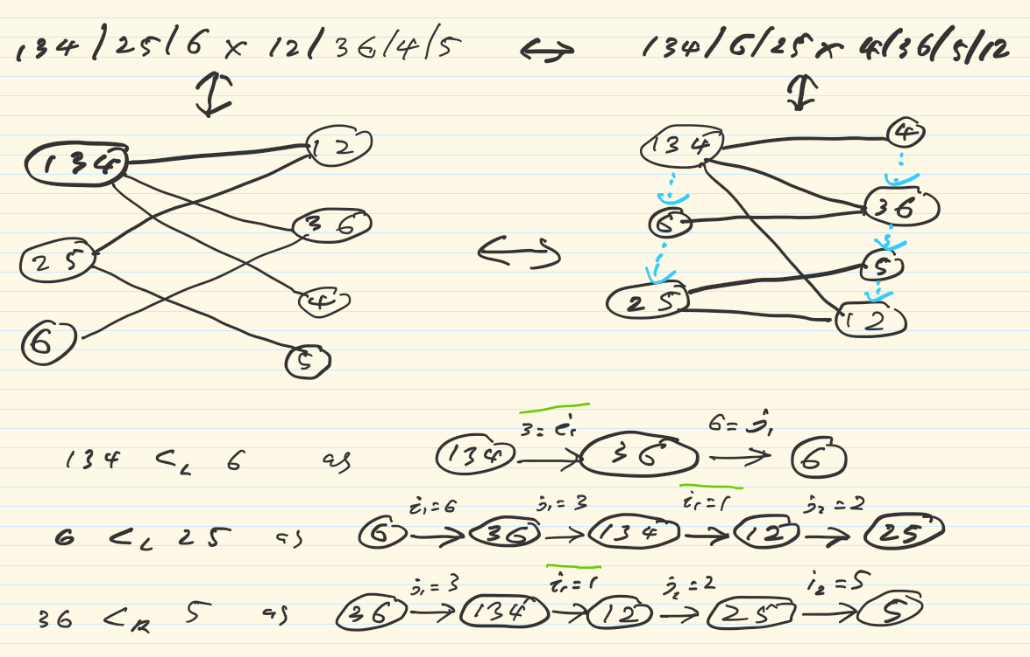
\includegraphics{Images/bijections_example.png}
\end{center}
\caption{The bijection between ordered partitions and bipartite trees.}
\end{figure}

\begin{corollary}[\cite{kajitani1982number}]
The number of essential complementary partitions is $|\EC_n| = 2(n+1)^{n-2}$.
\end{corollary}

\subsection{Bijection with the facets of the diagonal}

We denote by $\OP$ be the set of ordered pairs of partitions of $[n]$ labeling facets of the diagonal $\triangle$.

\begin{thm}
Facets of the diagonal and essential complimentary partitions are in bijection through the inverse functions $u:\OP \to \EC$ and $o:\EC\to \OP$, where
\begin{enumerate}
    \item The function $u$ forgets the order of the ordered partition pair.
    \item The function $o$ uniquely orders an essential complimentary partition pair via the defining conditions of the diagonal. 
\end{enumerate}
\end{thm}
We shall prove this theorem by establishing the necessary total order, showing that the functions are well defined, and then showing that they are injective.

\begin{lemma} 
\label{u well defined}
The function $u:\OP \to \EC$ that forgets the order in a pair of partitions is well defined.
\end{lemma}
\begin{proof}
Let $P \in \OP_n$. Then $G(u(P))$ is a graph with $l+r=n+1$ vertices, and $n$ edges. Furthermore, as no vertices can be isolated it must be the case that this graph is a tree. 
It is straightforward to verify that $G(u(P))$ must be labeled bipartite tree, but here is how we may explicitly produce the necessary distinct representatives using an algorithm of \cite[Theorem 2]{kajitani1982number}.

Let $G'$ be a copy of $G(u(P))$. 
While there is a vertex of degree $1$ in $G'$ delete it and add the sole edge of that vertex as a distinct representative of the corresponding partition of that vertex. 
As $G'$ is a tree this process can continue until there is a single edge connecting two vertices of degree $1$. 
This edge specifies the element $p$ of the distinct representatives.
\end{proof}

\begin{construction} 
\label{Order Lemma}
For $P=(P_L,P_R) \in \EC$ an essential complementary pair, we construct total orders on $P_L$ and $P_R$ in three steps:
\begin{enumerate}
    \item For $l,l' \in L$ there exists a unique minimal set of edges $p_{l,l'}$ of even cardinality connecting $V(P_l)$ and $V(P_{l'})$ in $G(P)$ (similar for $R$). We partition this set of edges as $I\cup J$ where $I$ and $J$ are each pairwise non-adjacent, and $I$ contains the minimal edge.
    \item Orient each path so that $I$ points left to right, and $J$ points right to left (same orientation for $P_L$ and $P_R$). 
    \item We say $P_l< P_{l'}$ (or $P_r < P_{r'}$) if the constructed path points from $V(P_l) \to V(P_{l'})$ ($V(P_r) \to V(P_{r'})$.
\end{enumerate}
\end{construction}

\begin{proof}
We first show our binary relation is well defined before verifying that it defines a total order on $G(P)$ and hence $P$ via the bijection of \cref{EC Graph Bijection}.

As $G(P)$ is a bipartite tree, every vertex is connected, and every path connecting two vertices on the same side must be of even length. 
As $I$ and $J$ are each pairwise non-adjacent, they must partition the path in an alternating fashion i.e. $p=(I_{i_1},J_{j_1},I_{i_2},J_{j_2},..., )$, hence we can orient the path by forcing $I$ to point left and $J$ to point right.

This order is clearly total, reflexive (by convention) and anti-symmetric, what remains to be checked is its transitivity. 
Let $p_{v,v'}$ denote the unique minimal path between two vertices and for a set $A$ let $A_*:= \min A$, in particular ${I_{v,v'}}_*$ denotes the minimal value of $I$ on this path. 
Suppose there exists three vertices $a,b,c$ all on the same side (either left or right) such that the following conditions hold.
\begin{align*}
    a<b \quad &\iff \quad {I_{a,b}}_* = ({I_{a,b}} \cup J_{a,b})_*\\
    b<c \quad &\iff \quad{I_{b,c}}_* = ({I_{b,c}} \cup J_{b,c})_*
\end{align*}
As $a,b,c$ are all vertices on a tree there must exist a middle vertex $m$ such that all unique minimal paths $p_{a,b},p_{b,c}$ and $p_{a,c}$ use this vertex (in general this vertex could be $b$). There are four possibilities for the joint locations of ${I_{a,b}}_*$ and ${I_{b,c}}_*$ which are illustrated in \cref{fig:transitivity-cases}.

\begin{figure}
\begin{center}
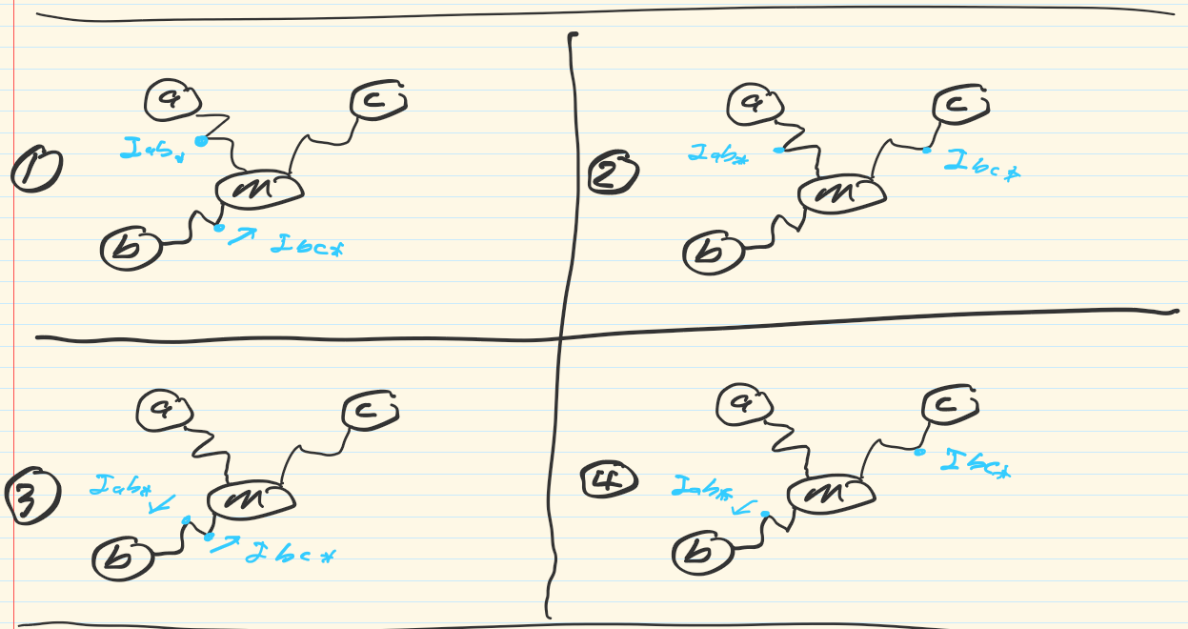
\includegraphics{Images/transitivity cases.png}   
\end{center}
\caption{Transitivity cases}
\label{fig:transitivity-cases}
\end{figure}

\begin{enumerate}
    \item Here ${I_{b,c}}_* \in J_{a,b}$ and hence ${I_{a,c}}_*={I_{a,b}}_*<{I_{b,c}}_*$.
    \item Here ${I_{a,c}}_* = ({I_{a,b}} \cup {I_{b,c}})_*$.
    \item Here we have a contradiction as ${I_{b,c}}_* \in J_{a,b} \implies {I_{a,b}}_*<{I_{b,c}}_*$  and ${I_{a,b}}_* \in J_{b,c} \implies {I_{b,c}}_*<{I_{a,b}}_*$.
    \item Here ${I_{a,b}}_* \in J_{b,c}$ and hence ${I_{a,c}}_*={I_{b,c}}_*<{I_{a,b}}_*$. 
\end{enumerate}
So, for every case except the contradictory $3$rd we have that \begin{align*}
    {I_{a,c}}_* = ({I_{a,b}} \cup J_{a,b} \cup {I_{b,c}} \cup J_{b,c})_* = ({I_{a,c}} \cup J_{a,c})_* \implies a < c 
\end{align*}
\end{proof}
\Kurt{An alternate proof given by Guillaume is the following, but I think we still might need to to handle the contradiction case in this. (or this fixed by something I'm not seeing?)}
\Guillaume{Here is my argument, it includes the contradiction case (it does not occur, by definition!)}

\begin{lemma}[Transitivity]
\end{lemma}
\begin{proof}
    Let $p_{ab}$ denote the unique maximal path between two vertices $a$ and $b$ on the left of $G(P)$, that is two blocks of $P_L$. 
    Let $I_{ab}$ denote the set of left-to-right edges in this path, and let $J_{ab}$ denote its complement. 
    Then, we have 
    \begin{equation}
        \label{eq:order}
        a < b \iff \min(I_{ab}\cup J_{ab})=\min(I_{ab}) \ . 
    \end{equation}
    Suppose now that $a < b$ and $b < c$.
    Since $p_{ac}= (p_{ab} \cup p_{bc}) \setminus (p_{ab} \cap p_{bc})$, we have $$ I_{ac}=(I_{ab}\cup I_{bc}) \setminus (J_{ab} \cup J_{bc}) \text{ and } J_{ac}=(J_{ab}\cup J_{bc}) \setminus (I_{ab} \cup I_{bc}) \ , $$ and from the condition \cref{eq:order} above it is clear that $\min(I_{ac}\cup J_{ac})=\min(I_{ac})$.
\end{proof}

This order far from being arbitrary provides the unique way to order an essential complimentary partition pair into an ordered partition pair of $\triangle$, as we shall demonstrate in the next lemma.

\begin{lemma} 
\label{o well defined}
The function $o:\EC \to \OP$ that orders an essential complimentary pair is well defined.
\end{lemma}

\begin{proof}
Let $P=(P_L,P_R) \in EC$ and consider $o(P)$. We first show that every $I,J \in D(n)$ which correspond to a path between vertices is satisfied. Suppose $I,J$ corresponds to a path between two vertices on the left, i.e.
\begin{align*}
    V(P_l) = V_{L_1} \xrightarrow{i_1} V_{R_1}\xrightarrow{j_1} V_{L_2} \xrightarrow{i_2}... \xrightarrow{i_{k}} V_{R_{k-1}} \xrightarrow{j_k} V_{L_k}=V(P_{l'})
\end{align*}
By construction we have that $I = \{i_1,...,i_k\},J=\{j_1,...,j_k\} \in D(n)$ (note we are ordering $I$ and $J$ by the path, so it is not necessarily the case that $\min I = i_1$). Furthermore, each sub partition of $P_R$ either contains a single element of $I$ and a single element of $J$, or it contains no elements of $I$ and no elements of $J$. As such for any ordering of the sub-partitions of $P_R$ we have that 
\begin{align*}
    \forall m, |\bigcup_{1\leq k \leq m} P_{R,k} \cap I| = |\bigcup_{1\leq k \leq m} P_{R,k} \cap J|
\end{align*}
Hence in order for this $D(n)$ condition to be satisfied it must be the case that for some ordering of the sub-partitions of $P_L$ that we have
\begin{align*}
    \exists m, |\bigcup_{1\leq k \leq m} P_{L,k} \cap I| > |\bigcup_{1\leq k \leq m} P_{L,k} \cap J|
\end{align*}
Every sub-partition of $P_L$ excluding the $l$th and $l'$th either contains no elements of both $I$ and $J$, or it contains a single element of $I$ and a single element of $J$. So the only way for the condition to be satisfied is for $P_l$ to come before $P_{l'}$, which is precisely what is required by the total order.
\\\\
If $I,J$ corresponds to a path between two vertices on the right,
\begin{align*}
    V(P_r) = V_{R_1} \xrightarrow{j_1} V_{L_1}\xrightarrow{i_1} V_{L_2} \xrightarrow{j_2}... \xrightarrow{j_{k}} V_{L_{k-1}} \xrightarrow{1_k} V_{R_k}=V(P_{r'})
\end{align*}
then a similar chain of logic implies we must have an ordering of the sub-partitions of $P_R$ such that
\begin{align*}
    \exists m, |\bigcup_{1\leq k \leq m} P_{R,k} \cap I| < |\bigcup_{1\leq k \leq m} P_{R,k} \cap J|
\end{align*}
and this can only happen if $P_r$ comes before $P_{r'}$.
\\\\
What remains to be shown is that every $I,J \in D(n)$ which does not correspond to a path is satisfied... 
\\\\
A likely proof method seems to be assume there exists such an $I,J$ which contradicts the $D(n)$ assumption then show this leads to contradiction....
\end{proof}

\begin{lemma} \label{o and u are injective}
Both $u:\OP \to \EC$ and $o:\EC\to \OP$ are injective, with the other function being their inverse.
\end{lemma}
\begin{proof}
The forgetful function $u$ is clearly the inverse to $o$ as forgetting any assigned order will clearly return the original essential complimentary partition pair. The ordering function $o$ is the inverse to $u$ as it returns the sole ordering of the sub-partitions which is compatible with the $D(n)$ conditions.
\end{proof}




\section{Vertices of the diagonal}

We are now interested in characterizing the pairs of vertices that occur in the diagonal, that is pairs of permutations $(\sigma_1,\sigma_2) \in \triangle$. 

\begin{thm} There exists $(I,J) \in D(n)$ such that $\forall k, |\sigma_1^1\cdots\sigma_1^k \cap I| \leq |\sigma_1^1\cdots\sigma_1^k \cap J|$ and $\forall l, |\sigma_1^1\cdots\sigma_1^l \cap I| \geq |\sigma_1^1\cdots\sigma_1^l \cap J|$ (diagonal condition) if and only if $\exists (I',J')=(\{i_1,\ldots,i_m\},\{j_1,\ldots,j_m\}) \in D(m)$, $m\leq n$, such that \[\sigma_1 \cap (I'\cup J')=j_1 i_1 j_2 i_2 \cdots j_n i_n \] and \[ \sigma_2 \cap (I'\cup J') = i_2 j_1 i_3 j_2 \cdots i_n j_{n-1} i_1 j_n \ , \] where $i_1 = \min (I' \cup J')$ (fish condition). 
\end{thm}

\begin{proof}
\begin{itemize}
\item If a pair of permutations $(\sigma_1, \sigma_2) \in   \mathfrak{S}_N^2$ satisfies the fish condition, then there exist two sets $I$ and $J$ of same cardinality such that $\min(I)<\min(J)$. Denoting $\sigma_1$ and $\sigma_2$ by two words of size $N$ $\sigma_1^1 \ldots \sigma_1^N$ and $\sigma_2^1 \ldots \sigma_2^N$, then the pair $((\sigma_1, \sigma_2), (I,J))$ satisfies that for any $k$ in $\llbracket 1;N\rrbracket$, $|\sigma_1^1 \ldots \sigma_1^k \cap J| \geq |\sigma_1^1 \ldots \sigma_1^k \cap I|$ and $|\sigma_2^1 \ldots \sigma_2^k \cap I| \geq |\sigma_2^1 \ldots \sigma_2^k \cap J|$, hence the diagonal condition.
\item We will now prove the converse. Let us presume that $(\sigma_1, \sigma_2)$ is a pair of permutations satisfying the diagonal condition for a pair of sets $(I,J) \in D(n)$, minimal for the inclusion of sets.
\begin{description}
\item[Case $n=1$] 
\end{description}
If $|I|=|J|=1$, then it follows directly from the diagonal condition above that ${\sigma_1}_{| I \cup J}=j_1 i_1$ and ${\sigma_1}_{|I \cup J}=i_1 j_1$, hence the fish condition is satisfied.
\begin{description}
\item[Case $n>1$] 
\end{description}
In this case, the proof is made by absurdum 
by considering the number of "well-placed" elements of $I$ and $J$ in $\sigma_1$ and $\sigma_2$. In what follows, for any set $E$, $\sigma^{E}_i$ will stands for $(\sigma_i)_{|E}$. We write also $n_{i,k}^E$ for the number of elements of $E$ in the $k$ first letters of $\sigma_i$. The main argument in each of the small proofs below is the same: if the permutations do not satisfy the pattern described above, then it is possible to find an appropriate pair of elements $(i,j)\in I \times J$ such that $(I-i,J-j)$ satisfies the diagonal condition, hence  contradicting the minimality of $(I,J)$.

We first prove that the leftmost element of $\sigma^{I}_1$ is $i_1$. Indeed, if it is not the case, we consider $i$, the leftmost element in $\sigma^{I}_1$ and $j$ the leftmost element in $\sigma^{J}_2$. The pair $(I-i,J-j)$ is in $D(n-1)$, as $i$ is different from $i_1$. Moreover, it is clear that the diagonal condition still holds for $((\sigma_1, \sigma_2), (I,J))$. As this would contradict the minimality of $(I,J)$, the leftmost element of $\sigma^{I}_1$ is $i_1$.

We then prove that $\sigma^{I \cup J}_1$ starts by $j_1 i_1$ and that this $j_1$ is exactly the leftmost element in  $\sigma^{J}_2$. On that purpose, we suppose that either  $i_1$ is preceeded by several elements of $J$ or that the unique element of $J$ is not the leftmost one in $\sigma^{J}_2$. We then adapt the previous argument by choosing $i$ to be the leftmost element in $\sigma^{I-\{i_1\}}_1$ and $j$ the leftmost element in $\sigma^{J}_2$. The pair $(I-i,J-j)$ is in $D(n-1)$. Let us briefly explain while  the diagonal condition would still be fulfilled in this case. If $j$ is after $i_1$ in $\sigma_1$, then the difference $n_{1,k}^{J-j}-n_{1,k}^{I-i}$ is greater than $n_{1,k}^{J}-n_{1,k}^{I}$ for any $k$, hence is non negative. If $j$ is before $i_1$ in $\sigma_1$, then by hypothesis, the difference $n_{1,k}^{J-j}-n_{1,k}^{I-i}$ is:
\begin{itemize}
\item strictly positive before $i_1$ an greater than $1$ just before $i_1$
\item non negative after $i_1$
\item increase between $i_1$ and $i$
\item is equal to $n_{1,k}^{J}-n_{1,k}^{I}$ after $i$,
\end{itemize} 
hence is always non negative.
Moreover, if $i$ is after $j$ in $\sigma_2$, the diagonal condition is clearly satisfied. If $i$ is before $j$, then the difference $n_{2,k}^{I-i}-n_{1,k}^{J-j}$ is:
\begin{itemize}
\item strictly positive before $j$ an greater than $1$ just before $j$
\item is equal to $n_{2,k}^{I}-n_{1,k}^{J}$ after $j$,
\end{itemize} 
hence is always non negative. In short, if $i_1$ is preceeded by several elements of $J$ or the unique element of $J$ is not the leftmost one in $\sigma^{J}_2$, we obtain a contradiction with the minimality of $(I,J)$.

Let us now consider the biggest $k\geq 1$ such that $\sigma^{I \cup J}_1$ begins with $j_1 i_1 j_2 i_2 \ldots j_k i_k$ and $\sigma^{I \cup J}_2$ begins with $i_2 j_1 i_3 j_2\ldots i_k j_{k-1} w j_k$, where $w$ is a word with letters in $I$. We want to show that $k=n$. Let us first remark that if $k=n$, $w=i_1$. If $1\leq k<n$, then the sets $\tilde{I}=I-\{i_1, \ldots, i_k\}$ and $\tilde{J}=J-\{j_1, \ldots, j_k\}$ are non empty. Let us choose $i_{k+1}$ to be the leftmost element in $\sigma^{\tilde{I}}_1$ and $j_{k+1}$ the leftmost element in $\sigma^{\tilde{J}}_2$. We thus have $\sigma^{I \cup J}_1=j_1 i_1 j_2 i_2 \ldots j_k i_k w' i_{k+1}\ldots$, where $w'$ is in $J$ and $\sigma^{I \cup J}_2= i_2 j_1 i_3 j_2\ldots i_k j_{k-1} w j_k w'' j_{k+1}\ldots $, where $w$ and $w'$ are words with letters in $I$. The pair $(I-i_{k+1},J-j_{k+1})$ is in $D(n-1)$. Following the study as in the previous case, $\sigma_1$ always satisfies the diagonal condition for $(I-i_{k+1},J-j_{k+1})$ and $\sigma_2$ satisfies it if and only if $w \neq i$. By minimality of $(I,J)$, we then have $w=i_{k+1}$. If $k+1=n$, we are done as the only possible word in $J$ is $j_{k+1}$, hence $w'=j_{k+1}$. Otherwise, we can choose $i_{k+2}$ to be the leftmost element in $\sigma_1^{\tilde{I}-i_{k+1}}$. Using the same reasoning as above, we show that $((\sigma_1, \sigma_2),(I-i_{k+2},J-j_{k+1}))$ satisfies the diagonal condition if and only if $w'\neq j_{k+1}$. To sum up, the only possibility for $(I,J)$ to be minimal is to have $k=n$, which implies the fish condition.
\end{itemize}
\end{proof}

\begin{corollary} For any pair of permutations $(\sigma_1, \sigma_2$, there exists $(I,J) \in D(n)$ such that $((\sigma_1, \sigma_2),(I,J))$ satisfies the diagonal condition if and only if there exists $(I',J') \in E(m)$, $m<n$ such that $((\sigma_1, \sigma_2),(I',J'))$ satisfies the fish condition, with 
\begin{multline}
E(m)=\{(I,J)\in D(m)| \min(J)<\min(I-\min(I)), |\llbracket 1; k \rrbracket \cap J| > |\llbracket 1; k \rrbracket \cap I| \\ \text{ if } |\llbracket 1; k \rrbracket \cap J| \geq 2 \text{ and } I \subsetneq \llbracket 1; k \rrbracket \}
\end{multline}
\end{corollary}

\begin{proof}
It follows directly from the fish condition: if the fish condition is satisfied, as inversions of $\sigma_1$ are included in inversions of $\sigma_2$, we get $j_{k-1},j_k<i_k$ for any $k>1$.
\end{proof}


\section{Tables}

In this section we present low dimensional computations of the enumeration results obtained above and we connect them to other known combinatorial objects. 

\begin{figure}[h]
\centerline{
\begin{tabular}{r|c}
\textbf{dim} & \textbf{0}  \\
\hline
\textbf{0} & 1  
\end{tabular}
\ \ \
\begin{tabular}{r|cc}
\textbf{dim} & \textbf{0} & \textbf{1}  \\
\hline
\textbf{0} & 3 & 1 \\
\textbf{1} & 1 &  
\end{tabular}
\ \ \
\begin{tabular}{r|ccc}
\textbf{dim} & \textbf{0} & \textbf{1} & \textbf{2}  \\
\hline
\textbf{0} & 17 & 12 & 1 \\
\textbf{1} & 12 &  6 & \\
\textbf{2} & 1 &  & 
\end{tabular}
\ \ \
\begin{tabular}{r|cccc}
\textbf{dim} & \textbf{0} & \textbf{1} & \textbf{2} & \textbf{3} \\
\hline
\textbf{0} & 149 & 162 & 38 & 1 \\
\textbf{1} & 162 & 150 & 24 & \\
\textbf{2} & 38 & 24 & & \\
\textbf{3} & 1 & & &
\end{tabular}
}
\caption{Number of pairs of faces in the cellular image of the diagonal $0$, $1$, $2$ and $3$-dimensional permutahedra.}
\label{t:dim1-3}
\end{figure}

\begin{figure}[h]
\centerline{
\begin{tabular}{r|ccccc}
\textbf{dim} & \textbf{0} & \textbf{1} & \textbf{2} & \textbf{3} & \textbf{4} \\
\hline
\textbf{0} & 1809 & 2660 & 1080 & 110 & 1 \\
\textbf{1} & 2660 & 3540 & 1200 & 80 & \\
\textbf{2} & 1080 & 1200 & 270 & & \\
\textbf{3} & 110 & 80 & && \\
\textbf{4} & 1 & & & &
\end{tabular}
\ \ \
\begin{tabular}{r|cccccc}
\textbf{dim} & \textbf{0} & \textbf{1} & \textbf{2} & \textbf{3} & \textbf{4} & \textbf{5} \\
\hline
\textbf{0} & 28399 & 52635 & 30820 & 6165 & 302 & 1 \\
\textbf{1} & 52635 & 90870 & 67580 & 7785 & 240 & \\
\textbf{2} & 30820 & 47580 & 20480 & 2160 & & \\
\textbf{3} & 6165 & 7785 & 2160 & && \\
\textbf{4} & 302 & 240 & & &&\\
\textbf{5} & 1 & & & &&
\end{tabular}
}
\caption{Number of pairs of faces in the cellular image of the diagonal $4$ and $5$-dimensional permutahedra.}
\label{t:dim4-5}
\end{figure}



\begin{figure}[h]
\centerline{\begin{tabular}{c|c|rrrrrrr|l}
\textbf{Pairs $(F,G) \in \Ima\triangle_{(P,\vec v)}$} & \textbf{Polytopes} & \textbf{0} & \textbf{1} & \textbf{2} & \textbf{3} & \textbf{4} & \textbf{5} & \textbf{6} & \textbf{\cite{OEIS}} \\
\hline
& \text{Associahedra} & 1 & 2 & 6 & 22 & 91 & 408 & 1938 & \OEIS{A000139}  \\
$\dim F + \dim G = \dim P$  & \text{Multiplihedra} & 1 & 2 & 8 & 42 & 254 & 1678 & 11790 &  to appear \\
  & \text{Permutahedra} & 1 & 2 & 8 & 50 & 432 & 4802 & 65536 &  \OEIS{A007334} \\
\hline
  & \text{Associahedra} & 1 & 3 & 13 & 68 & 399 & 2530 & 16965 &  \OEIS{A000260} \\
  $\dim F=\dim G =0$ & \text{Multiplihedra} & 1 & 3 & 17 & 122 & 992 & 8721 & 80920 & to appear \\
  & \text{Permutahedra} & 1 & 3 & 17 & 149 & 1809 & 28399 & 550297 &  \OEIS{A213507} 
\end{tabular}}
\caption{Number of pairs of faces in the cellular image of the diagonal of the associahedra, multiplihedra and permutahedra of dimension $0\leq \dim P \leq 6$, induced by any good orientation vector.}
\label{table:numerology}
\end{figure}


\emph{Acknowledgements.}    

\bibliographystyle{amsalpha}

\bibliography{Poissons}

\end{document}